\documentclass[aps,prl,floatfix,preprint,nofootinbib]{revtex4}
\usepackage{amsmath}
\usepackage{graphicx}
\usepackage[colorinlistoftodos]{todonotes}
\usepackage{indentfirst}
\usepackage{listings}
\usepackage{color}
\usepackage[title,titletoc,toc]{appendix}
\usepackage[hidelinks,hyperfootnotes=false,bookmarks=false]{hyperref}
\usepackage{epsfig}
\usepackage{setspace}

\setlength{\paperheight}{11in}

\input{formatting}

\begin{document}
\title{Modeling Two Body Collisions with Spring Potential Interactions}
\author{Matthew \textsc{Epland}, Douglas \textsc{Davis}}
\affiliation{Department of Physics, Duke University}
\date{\today}

\hypersetup{pdftitle=Modeling Two Body Collisions}
\hypersetup{pdfauthor={Matthew Epland, Douglas Davis}}
%\hypersetup{bookmarks=false}
\hypersetup{pdfkeywords={Classical Physics, Two Body Collisions}}

\begin{abstract}
This paper describes a computational study of two body collisions where the dynamics of the bodies are governed by a Hooke's Law type force at the interaction points. We investigate a number of scenarios which involve both a stationary target mass which is stuck by a projectile mass with some horizontal velocity in a two dimensional plane, as well as scenarios where both masses are moving in towards each other. The masses trajectories are determined from a simulation software package, written by the authors, that models the force between the masses as they interact with each other based on the initial kinematic state of the system. Specific attention was given to the systems behavior with different initial projectile velocities, impact parameters, energy loss rates and power dependence in the force law.
\end{abstract}\maketitle
\section{Introduction}
When two classical objects physically collide they experience a normal force between them. In the simplest case, that of two spherical masses, the normal force is orthogonal to the surface and is in line with the center of mass for both the objects. The magnitude of the normal force between masses $m_{1}$, $m_{2}$ with radii $r_{1}$, $r_{2}$ can be modeled as $ \left| F \right| = k \left(\Delta x\right)^{\lambda}$, where $\Delta x = r_1 + r_2 - \left| \mathbf{x}^{(1)}-\mathbf{x}^{(2)} \right|$ is the displacement from equilibrium and $k$ is an effective spring constant. Setting $\lambda = 1$ results in the familiar Hook's Law spring force, but by including the $\lambda$ power dependence we are able to study a wider array of collisions, particularly those where the masses deform enough that the normal force between them becomes nonlinear. As the masses deform and push against each other some of the mechanical energy of the system may be lost to internal degrees of freedom, such as heat. One way to model these inelastic collisions is by including viscous damping proportional to the velocity, which was the method used in this study.

Any two body collision can be reduced to 2-dimensional motion in a plane containing both masses and their initial velocity vectors. Additionally, in this paper we limit ourselves to the case where the initial velocities are parallel, though the masses may be initially off center from each other by a distance $s$, the impact parameter. One of the masses, the target $m_{1}$, may be at rest initially, though we also allow it to have an initial closing velocity in some studies. For continence we pick our coordinate system such that all the initial velocities lie along $\hat{x}$ and the target is on the $\hat{y}$ axis, $y_{1}(t=0)=0$ (Figure~\ref{fig:schematic}).

\begin{figure}[htbc]
	\centering
	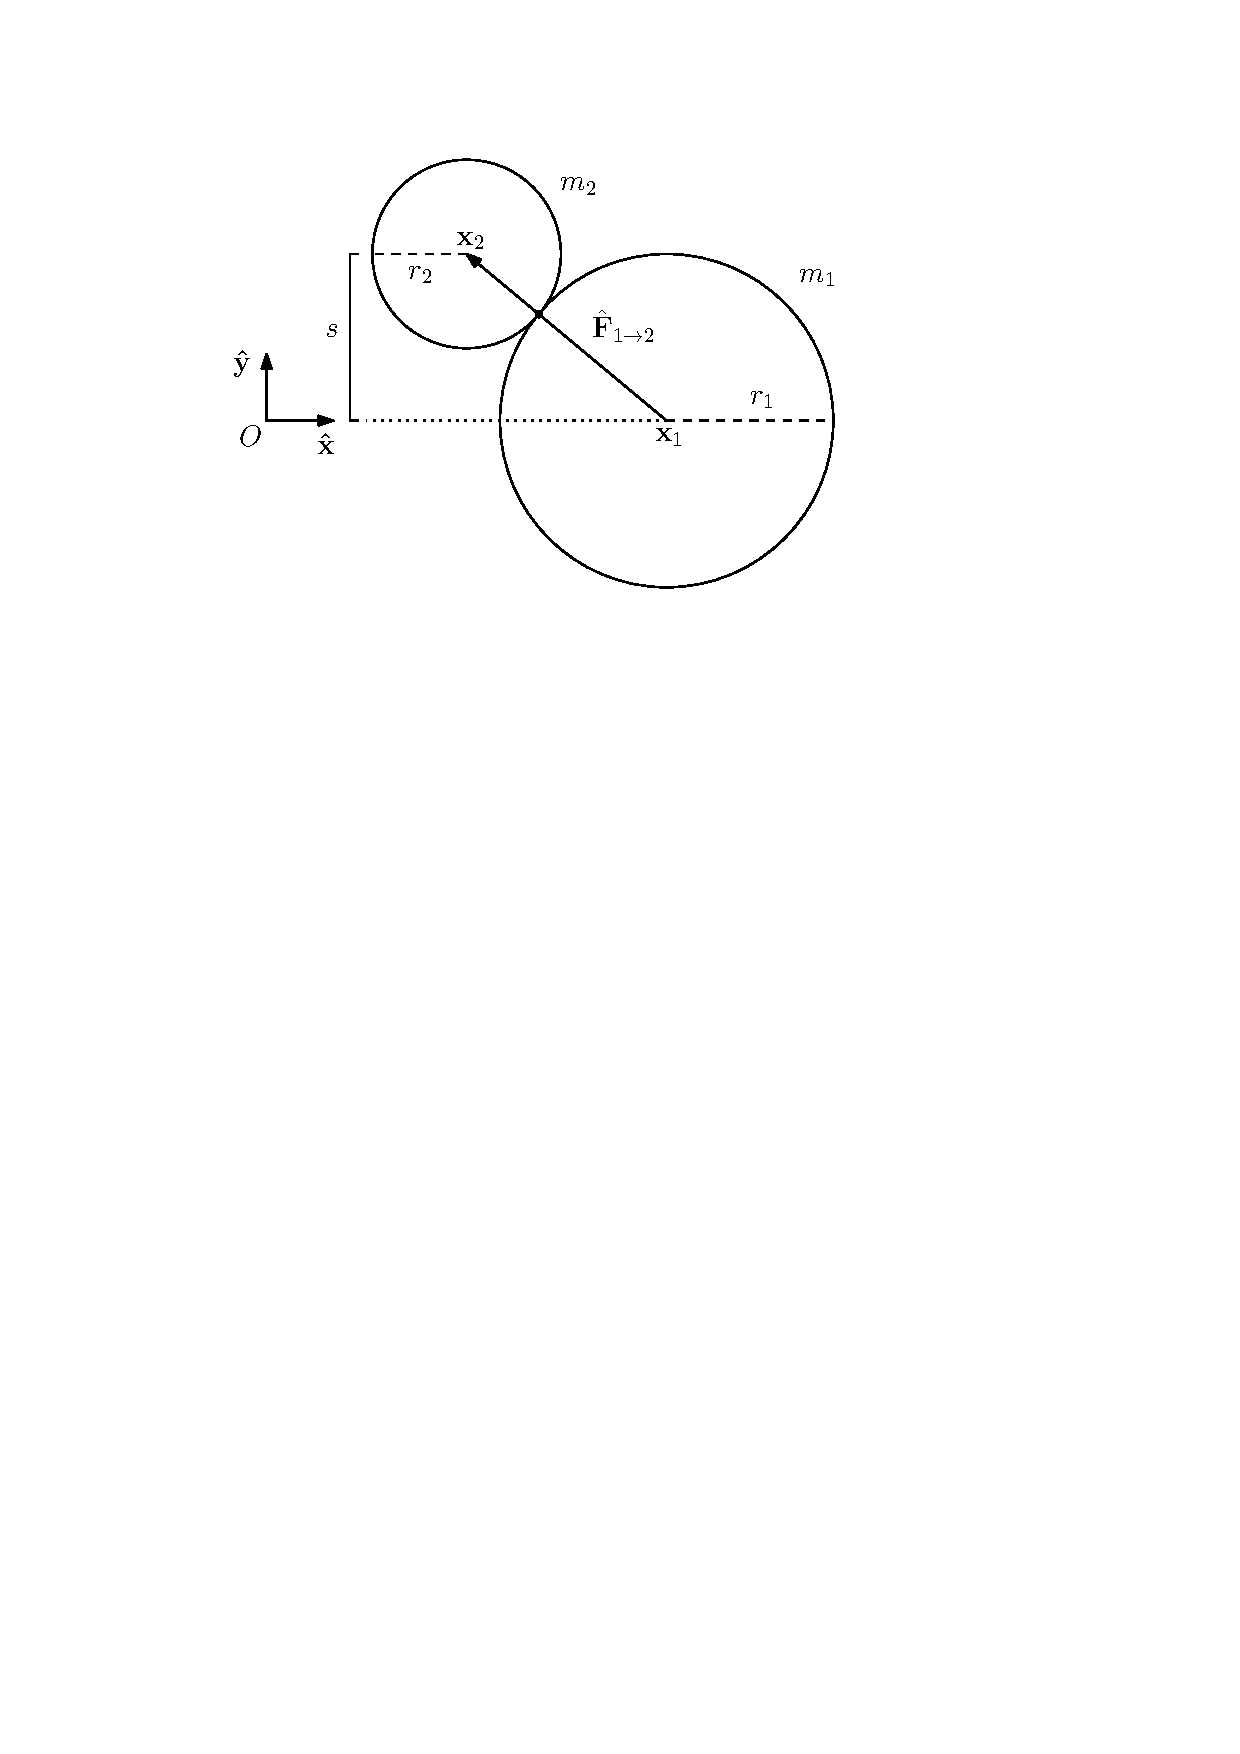
\includegraphics[width=.75\textwidth]{plots/cj_diag.pdf}
	{\par\nobreak\rule[9pt]{35em}{0.5pt}\vspace{-5mm}}
	\caption{Schematic View of the initial state at first contact, $t = 0$.}
	\label{fig:schematic}
\end{figure}

In order to rapidly investigate the many possible variations of this seemingly simple two body collision a software simulation was chosen over attempting to solve each variation analytically. Written in C++ and using some of the ROOT particle physics analysis libraries the simulation code at its core operates by iteratively calculating the masses change in position and velocity during a small time step, $\Delta t$, during which the acceleration is assumed to be constant. This is done by calculating $\Delta x$ \eqref{eq:displacement} from the $n-1$ positions, and then $\left|F\right|$ and the unit vector between the two masses centers $\hat{F}_{j\text{ on }i}$ \eqref{eq:force}. Once the force has been estimated it is a simple matter to compute the $n$ time step positions \eqref{eq:position}, and velocities \eqref{eq:velocity}. When calculating the velocity we include a $\left(1-\eta\right)$ term to implement the viscous dampening energy losses were $\eta$ is the proportional decrease in velocity per time step.

\begin{equation}\label{eq:position}
\mathbf{x}^{(i)}_{n} = \mathbf{x}^{(i)}_{n-1} + \dot{\mathbf{x}}^{(i)}_{n-1} \Delta t + \frac{1}{2m_i} \left| F \right| \mathbf{\hat{F}}_{j\text{ on }i} \left(\Delta t\right)^2
\end{equation}
\begin{equation}\label{eq:velocity}
\dot{\mathbf{x}}^{(i)}_{n} = (1-\eta)\dot{\mathbf{x}}^{(i)}_{n-1} + \frac{1}{m_i} \left| F \right| \mathbf{\hat{F}}_{j\text{ on }i} \Delta t
\end{equation}
\begin{equation}\label{eq:displacement}
\Delta x_{n-1} = r_1 + r_2 - \left| \mathbf{x}^{(1)}_{n-1}-\mathbf{x}^{(2)}_{n-1} \right|
\end{equation}
\begin{equation}\label{eq:force}
\left| F \right| = k \left(\Delta x_{n-1}\right)^{\lambda},\quad \mathbf{\hat{F}}_{j\text{ on }i} = \frac{\mathbf{x}^{(i)}_{n-1}-\mathbf{x}^{(j)}_{n-1}}{\left|\mathbf{x}^{(i)}_{n-1}-\mathbf{x}^{(j)}_{n-1}\right|}
\end{equation}

In addition to the position and velocity of the masses we also calculate their kinetic energies and the potential energy stored in the deformed bodies, e.g. spring \eqref{eq:energy}. The force is conservative, so $\mathbf{F} = - \nabla V \rightarrow V = \int \left|F\right| dx$. With a small enough $\Delta t$ these iterative equations model the physics of the interaction very well. 
\begin{equation}\label{eq:energy}
V_n = \frac{k}{\lambda+1}\left(\Delta x_n\right)^{\lambda+1},\quad T_n = \frac{m_1}{2}\left(\dot{\mathbf{x}}^{(1)}_n\right)^2 + \frac{m_2}{2}\left(\dot{\mathbf{x}}^{(2)}_n\right)^2
\end{equation}

\section{Results}
\subsection{Simulation Performance}
The simulation was good, here's why - include the single event plots

\subsection{Initial Velocity Studies}
The

\subsection{Impact Parameter Studies}
The

\subsection{Force Power Law Dependence}
The

\subsection{Energy Dissipation Studies}
The

\section{Conclusion}
The

\clearpage
\begin{appendices}
\singlespacing
\section{main.cpp} \label{sec:main}
%\lstinputlisting{main.cpp}% lots of pages, only uncomment when you want it
% use [firstline=, lastline=] to select only the physics loop

\end{appendices}




\end{document}
